%----------------------------------------------------------------------------
\chapter{Automatizált feladatkiértékelő modul}\label{chapter:exercise}
%----------------------------------------------------------------------------

A JPorta egyik fő funkciója a beadott feladatmegoldások automatikus kiértékelése. Ennek implemenetációja során törekedtek az általános, könnyen bővíthető megoldás megtalálására, amikkel akár nem programozási jellegű feladatokat is ki lehet adni. \cite{DudiMsc}

Az elkészült modul blokkokból épül fel, melyek egy-egy kiértékelési feladatot valósítanak meg. Ennek köszönhetően új igény esetén nem kell a meglévő blokkokat módosítani, csak az új funkciót megvalósító blokkot létrehozni.

A blokkok közötti kommunikációt bemeneti és kimeneti csatlazkóik teszik lehetővé. Ezek szabadon összeköthetőek bármely más blokk ellenkező típusú csatlakozójával, pl. a felhasználói fájl blokk kimenetét ráköthetjük a GCC fordító blokk bemenetére, így lefordíhatjuk az adott forrásfájlt (blokkok típusait lásd lentebb). Ezen kívül lehetnek olyan paraméterei is egy blokknak, melyeket adminisztrátori felületen kell beállítani, pl. fordítás esetén a fordítónak átadott kapcsolók.

Ilyen meglévő blokkok a következők:

\begin{itemize}
    \item Specifikáció blokk: tartalmazza a feladat leírását, akár hallgató specifikus elemekkel (pl. neptun kód, név, egyedileg generált szám, stb.). 
    \item Felhasználói fájl blokk: hallgatói megoldásként feltöltött fájl.
    \item GCC fordító blokk: forrásfájlok fordítását végzi GCC fordítóval (\ref{fig:exercise_blokk}. ábra).
    \item Futtató blokk: futtatható fájlokat képes futtatni, kimeneteiket továbbítani.
    \item Szöveges ellenőrző blokk: bemenetén kapott szövegek összehasonlítását teszi lehetővé.
    \item Szkript ellenőrző blokk: különböző szkript nyelveken írt ellenőrzést tesz lehetővé, stb.
\end{itemize} 

\begin{figure}[p]
    \centering
    \resizebox{\textwidth}{!}{
        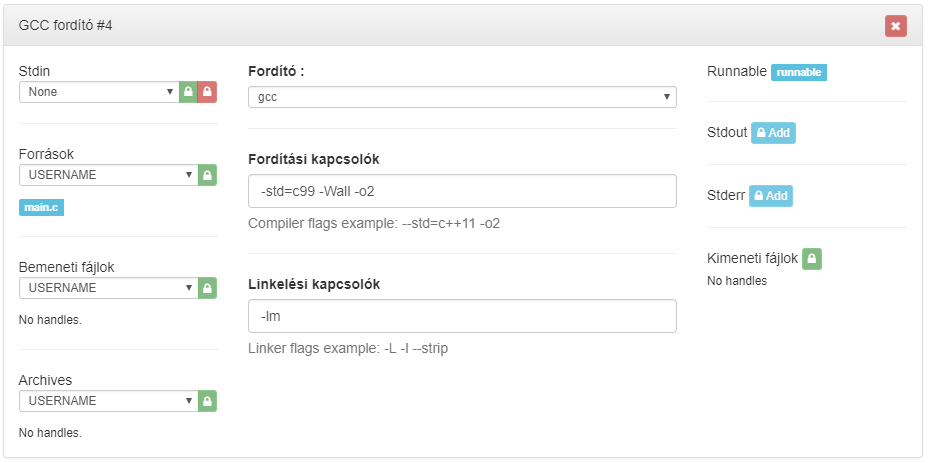
\includegraphics[]{exercise_blokk.png}
    }
    \caption{GCC fordító blokk adminisztrációs felülete}
    \label{fig:exercise_blokk}
\end{figure}

\section{Jogosultságok felülvizsgálata (2-3 oldal)}\label{subsection:permissions}
Acl, django permissions, stb...

\section{Kód lefedettség ellenőrzés (2-3 oldal)}

\section{Feladatok (tesztek) importálása és exportálása (2-3 oldal)}

\section{Feladatok csoportosítása (2 oldal)}

\section{További lehetőségek}

\subsection{Plágiumkeresés (1-2 oldal)}

\subsection{Verziókezelő támogatás (1-2 oldal)}